\documentclass{beamer}

\usepackage[utf8x]{inputenc} %arregla tema tildes y ñ
\usepackage[activeacute,spanish]{babel}
\usepackage{tikz}
\usepackage{wrapfig} % para meter fotitos volando por ahí

\usetikzlibrary{arrows,shapes,arrows,chains,matrix}
%\usepackage[pdftex]{color}

%Tema
\usetheme{Warsaw}
%\usetheme{Berlin}


%\tikzstyle{blockPeque} = [rectangle, draw, thick,draw=gray!80,fill=gray!20,
%text width=80px, text centered, rounded corners, minimum height=13px,node distance = 3cm]

%Portada
\title{RF$^{2}$ - Recarga Fácil por Radio Frecuencia}
\author{Daniel Aicardi, Melina Rabinovich, Edgardo Vaz} 
\institute{
	Tutores: Ing. Juan Pablo Oliver, Ing. Andrés Aguirre\\

\bigskip
\bigskip
	Facultad de Ingeniería - UdelaR\\
	
	\bigskip
	
\includegraphics[scale=.2]{Imagenes/logos.jpg} \\%remove this line if no logo.
}

\date{\today}

\begin{document}

%Portada
\begin{frame}[plain]
	\titlepage
\end{frame} 


\begin{frame}\frametitle{Esquema de la presentaci\'on}
	\scriptsize 
	\tableofcontents
\end{frame}


%esto es para ejemplo nomás
\section{Introducción}

\subsection{Sistema de Transporte}
\begin{frame}

%	\begin{wrapfigure}{r}{3.5cm}
%		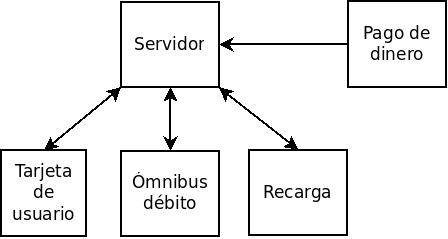
\includegraphics[width=3.5cm, scale=.5]{Imagenes/sistrans.jpg}
%	\end{wrapfigure}
	
	\begin{itemize}
		\item el pasajero usa su tarjeta como método de pago
		\item dispositivo lector a bordo que debita viajes
		\item recargar tarjetas
		\item sistema de gestión de negocios (servidores, seguridad, puntos de venta)
	\end{itemize}
\end{frame}

\begin{frame}
	\frametitle{Recarga hoy}
	
	Al día de hoy:
	\begin{itemize}
		\item mundo PC
		\item puntos de venta concentrados
		\item pago no desacoplado de la recarga
		\item no está pensado 24/7		
	\end{itemize}
\end{frame}

\begin{frame}
	\frametitle{Solución alternativa}
	
	Alternativa:
	\begin{itemize}
		\item mundo sistemas embebidos
		\item puntos de venta bien distribuídos
		\item pago desacoplado de la recarga
		\item 24/7		
	\end{itemize}
\end{frame}


%\subsection{Campos de aplicación}
%\begin{frame}
%	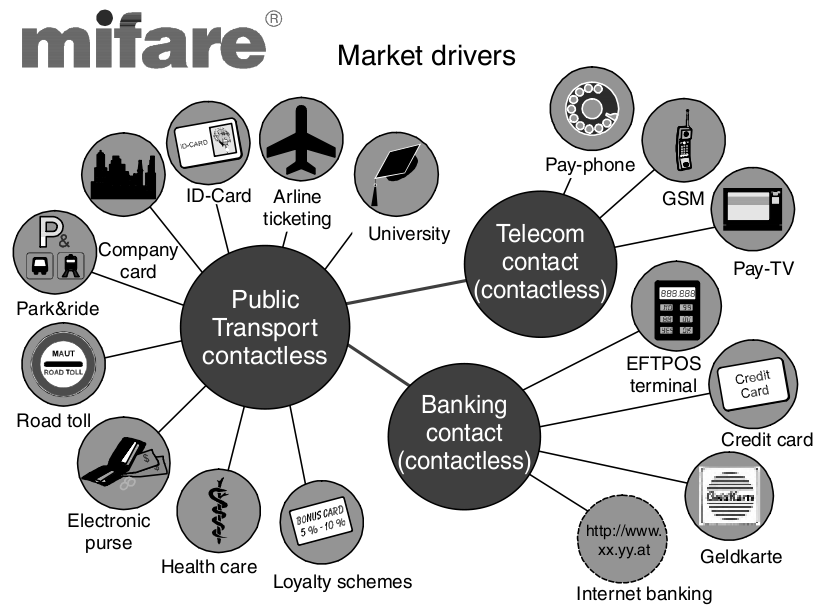
\includegraphics[scale=.4]{Imagenes/aplicaciones.png}
%\end{frame}


%%%%%%%%%%%

\section{Preguntas}
\begin{frame}
	\begin{center}
		\bigskip		
		
\includegraphics[scale=.5]{Imagenes/preg.jpg}
	\end{center}
\end{frame}

\end{document} 